\section{Requirements}
\label{section:requirements}

The requirements for our software stem from the growing need for parallel
analysis in the domain of climate science\cite{MODSIM07:LOT} but also from
the use of the geodesic grid.

\subsection{Geodesic Grid}

The data we work with comes from a climate model using a geodesic grid.  The
geodesic grid is created by recursively bisecting an icosahedron of 20
triangular faces and twelve vertices and projecting the resulting faces onto
a unit sphere.  The resulting vertices represent the centers of hexagonal grid
cells with the exception of twelve pentagons (the centers of the original
twelve vertices.)  Further details can be found in \cite{GEODESIC}.

\begin{figure}[!t]
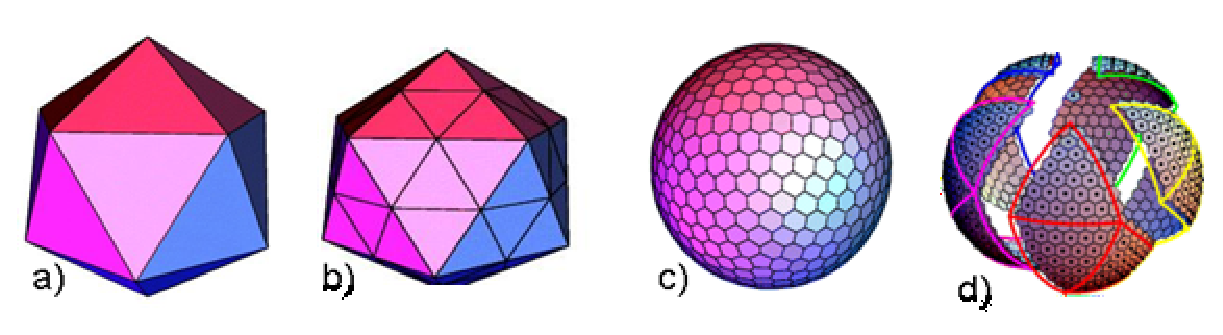
\includegraphics[width=2.5in]{images/geodesic.eps}
\caption{Geodesic decomposition and data layout TODO}
\label{fig:geodesic}
\end{figure}

Although the geodesic grid is fairly structured, we choose to represent it in
an unstructured way.  Each of the grid's cells, vertices, and edges are
uniquely indexed from zero.  For a given positive integer $R$, there are $N =
10 \times 2^{2R} + 2$ cells, $C = (N-2) \times 2$ corners, and $E = (N-2)
\times 3$ edges.  Increasing the value of $R$ increases the resolution of the
model.  For example, a value of $R=10$ is approximately 8Km while $R=11$ is
approximately 4Km.

Each cell, vertex, and edge has an associated longitude and latitude value
such that there are six one-dimensional arrays, \verb=grid_center_lat(cells)=,
\verb=grid_center_lon(cells)=, \verb=grid_corner_lat(corners)=,
\verb=grid_corner_lat(corners)=, \verb=grid_edge_lat(edges)=, and
\verb=grid_edge_lat(edges)=.  There are additional two-dimensional
index-mapping arrays associating cells to corners and cells to edges as well
as from edges to corners.  The vast majority of cells are hexagons, so we have
\verb+cell_corners(cells,cellcorners=6)+,
\verb+cell_edges(cells,celledges=6)+, and
\verb+edge_corners(edges,edgecorners=2)+.  For the twelve pentagons, the last
values in these arrays are repeated but could just have easily been set to a
negative index.  These variables represent the grid and are hereafter referred
to as grid variables.

Data variables make up the remained of what is stored.  In the horizontal
direction, data can be associated with either cells, corners, or edges.  In
the vertical direction, data can be associated with either a layer or the
interfaces between layers.  For example, the data variables
\verb+pressure(time,cells,layers)+ or \verb+wind(time,corners,interfaces)+.

\subsection{Data Parallelism}

Larson, Ong, and Tokarz note that the current popular climate data analysis
packages remain single-processor applications which lack the memory required
to handle the large data volumes as well as the processing power to analyse
the data in a timely fashion.\cite{MODSIM07:LOT}  Although they emphasize
using OpenMP as a first step toward parallism, we instead emphasize using the
message-passing model first.  Well designed message-passing libraries such as
MPI may already take advantage of shared-memory parallelism within a compute
node or multi-core desktop computer.

The data parallelism offered by libraries such as MPI or Global Arrays is
absolutely necessary to handle the size of data of modern climate models.  An
edge data variable of the geodesic grid at an approximate resolution of 2Km
and 100 levels is nearly $10 \times 2^{2R} \times 3 \times 100 \times 4
\unit{bytes} \approx 50 \unit{gigabytes}$ in size.  Even a modest number of
these variables will surpass most desktop and even some small clusters.

\subsection{Fast IO}

Efficiently reading and writing data of this size to disk requires the use of
parallel IO libraries such as the Parallel NetCDF\cite{PNETCDF} or the
HDF5/NetCDF4\cite{HDF5}\cite{NETCDF} libraries, both of which are in turn
built on top of the MPI-IO libraries\cite{MPIIO}.  Model output is stored in
netCDF\cite{NETCDF} files, a format for storing array-oriented
machine-independent data.  The use of Parallel NetCDF was selected because the
work on the HDF5/NetCDF4 was incomplete at the time of developement.

\subsection{Dataset Abstraction}

Model output is often distributed across many files for a given model run.
The reconstitution of these files into a logical set of variables and metadata
is an established practice.\cite{NcML}\cite{THREDDS}  We emphasize that the
aggregation of files into an abstract dataset is required in order to
operate on the data itself.

TODO -- Datasets, Variables, ConnectivityVariables,
Masks(?)

\subsection{Maintenance of Topology Variables}

Regular grids such as the cartesian, rectilinear, or curvilinear lend
themselves to representations as multidimensional arrays such that logically
adjacent cells are either adjacent in memory or can be located via a
shape-based index calculation.  Although some attempt is made to keep
logically adjacent cells nearby in memory, geodesic grids do not have the
luxury of using relatively simple shape-based index arithmetic to locate
neighbors.

\subsection{Maintain Integrity of Entire Grid Cells}

TODO -- In order for other applications to better use the data (i.e. viz).
